%%%%%%%%%%%%%%%%%%%%%%%%%%%%%%%%%%%%
% Header                           %
%%%%%%%%%%%%%%%%%%%%%%%%%%%%%%%%%%%%
% 
% Revisions: 2017-04-10 Martin R�del <martin.raedel@dlr.de>
%                       Initial draft
%               
% Contact:   Martin R�del,  martin.raedel@dlr.de
%            DLR Composite Structures and Adaptive Systems
%          
%                                 __/|__
%                                /_/_/_/  
%            www.dlr.de/fa/en      |/ DLR
% 
%%%%%%%%%%%%%%%%%%%%%%%%%%%%%%%%%%%%
% Content                          %
%%%%%%%%%%%%%%%%%%%%%%%%%%%%%%%%%%%%

\levelstay{Force-displacement-plots}

\leveldown{General}

This plot shows the course of the ``nodal'' force in a constrained region of the model over the displacement of a discrete point. The sum of the forces is used as a representative of the integral force value a load cell would show. For the displacement the value of a discrete node or collocation point is used as a representative for the scalar value of an extensiometer or the machine displacement value.

\levelstay{\protect\toolname/\protect\paraviewname}

\leveldown{Requisition of output values in \protect\toolname}

To acquire forces and displacements for a defined part of a model \texttt{Compute Class Parameters} are used in \toolname. They are described in sections \ref{sec:Peridigm:QRG:ComputeClassParameters:Nodeset}, \ref{sec:Peridigm:QRG:ComputeClassParameters:Block} \& \ref{sec:Peridigm:QRG:ComputeClassParameters:NearestPoint}. The forces are requested for the node set or block where a body load or in this case boundary condition is applied on. The displacement is written for one point in this node set using the nearest neighbor approach to a defined spatial coordinate in the node set region. The initial position of the point the displacements are written for is also requested for convenience and checks.

\begin{code}
Compute Class Parameters
  Strain Gage Initial Position
    Compute Class "Nearest_Point_Data"
    X 0.0317
    Y 1.238
    Z 0.0
    Variable "Model_Coordinates"
    Output Label "Gage_Initial_Position"
    Verbose "True"
  Strain Gage Displacement
    Compute Class "Nearest_Point_Data"
    X 0.0317
    Y 1.238
    Z 0.0
    Variable "Displacement"
    Output Label "Gage_Displacement"
    Verbose "True"
  Reaction Force
    Compute Class "Node_Set_Data"
    Calculation Type "Sum"
    Node Set "bc_load"
    Variable "Force"
    Output Label "Reaction_Force"
\end{code}

Alternatively, it should also be possible to request the displacement for the same node set as the force and simply choose ``Minimum'' or ``Maximum'' as \textit{Calculation type}. This way, it is not required to adjust the spatial coordinates as in \textit{Compute Class ``Nearest\_Point\_Data''}. This works fine for a test case.

Additionally the global output variable types \textit{Displacement} and \textit{Force} must be requested in the output section.

\begin{code}
Output
  Output File Type "ExodusII"
  Output Filename "model"
  Output Frequency 1
  Output Variables
    ...
    Displacement "true"
    ...
    Force "true"
    ...
    Gage_Initial_Position "true"
    Gage_Displacement "true"
    Reaction_Force "true"
\end{code}

\levelstay{Access result data in \protect\paraviewname}

\begin{figure}[htbp]
\centering
  \begin{subfigure}{0.49\linewidth}
    \centering
    \begin{tikzpicture}
      % External figure
      \node[anchor=south west,inner sep=0] (image) at (0,0) {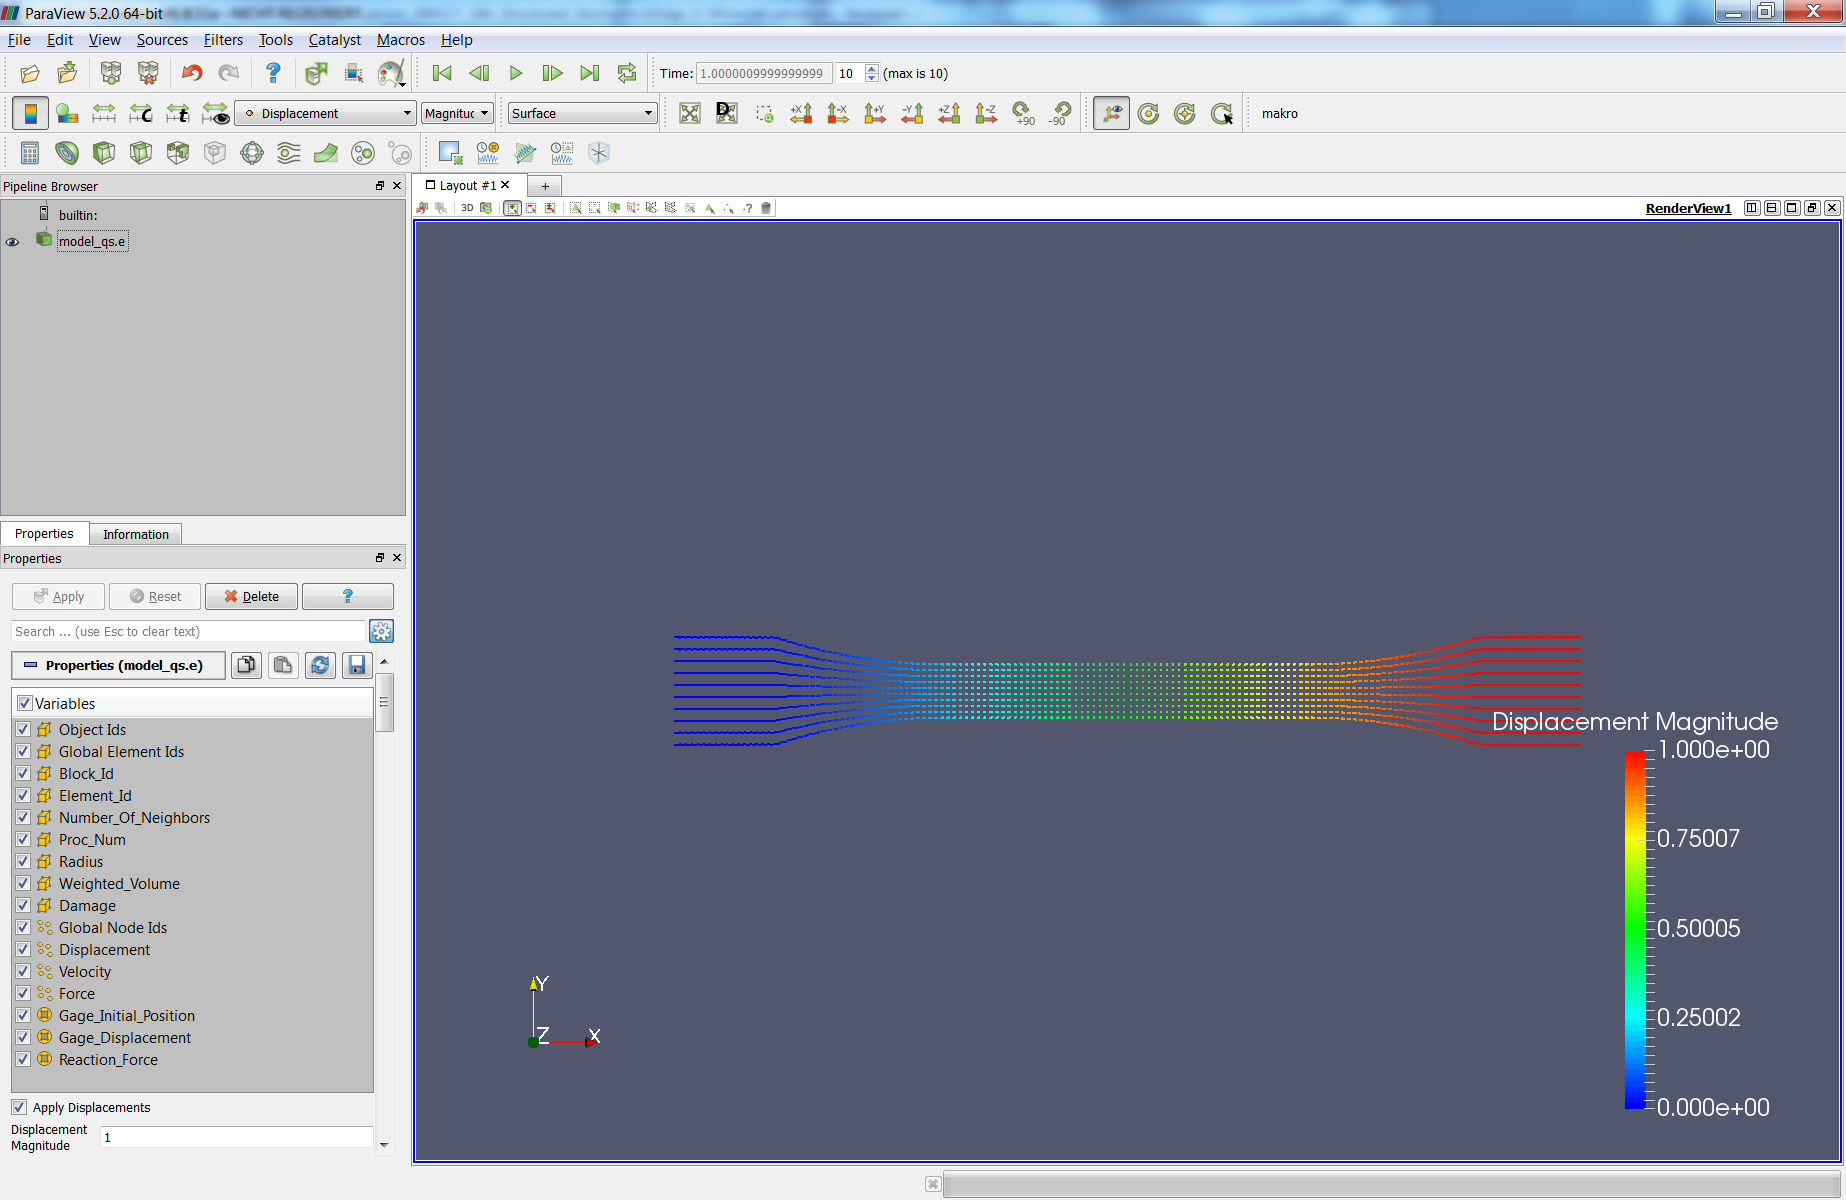
\includegraphics[width=\linewidth]{Figures/Screenshots/ParaView_ComputeClassParameter_ResultsData_1}};
      \begin{scope}[
        x={(image.south east)},
        y={(image.north west)},
      ]
        % Some label
        \node[fit={(0.007,0.10) (0.18,0.17)},myrectangularmarkup] (rect1) {};
        \node[anchor=west,mymarkuptext] (rect1label) at (rect1.east) {1};
        %
        \node[fit={(0.280,0.83) (0.31,0.86)},myrectangularmarkup] (rect2) {};
        \node[anchor=west,mymarkuptext] (rect2label) at (rect2.east) {2};
        % Help grid and labels
        %\pic{myimagegrid};
      \end{scope}
      % Outside label
    \end{tikzpicture}
    \caption{Steps 1-2}
    \label{fig:ParaView_ComputeClassParameter_ResultsData_1}
  \end{subfigure}%
  %\\
  \hfill
  \begin{subfigure}{0.49\linewidth}
    \centering
    \begin{tikzpicture}
      % External figure
      \node[anchor=south west,inner sep=0] (image) at (0,0) {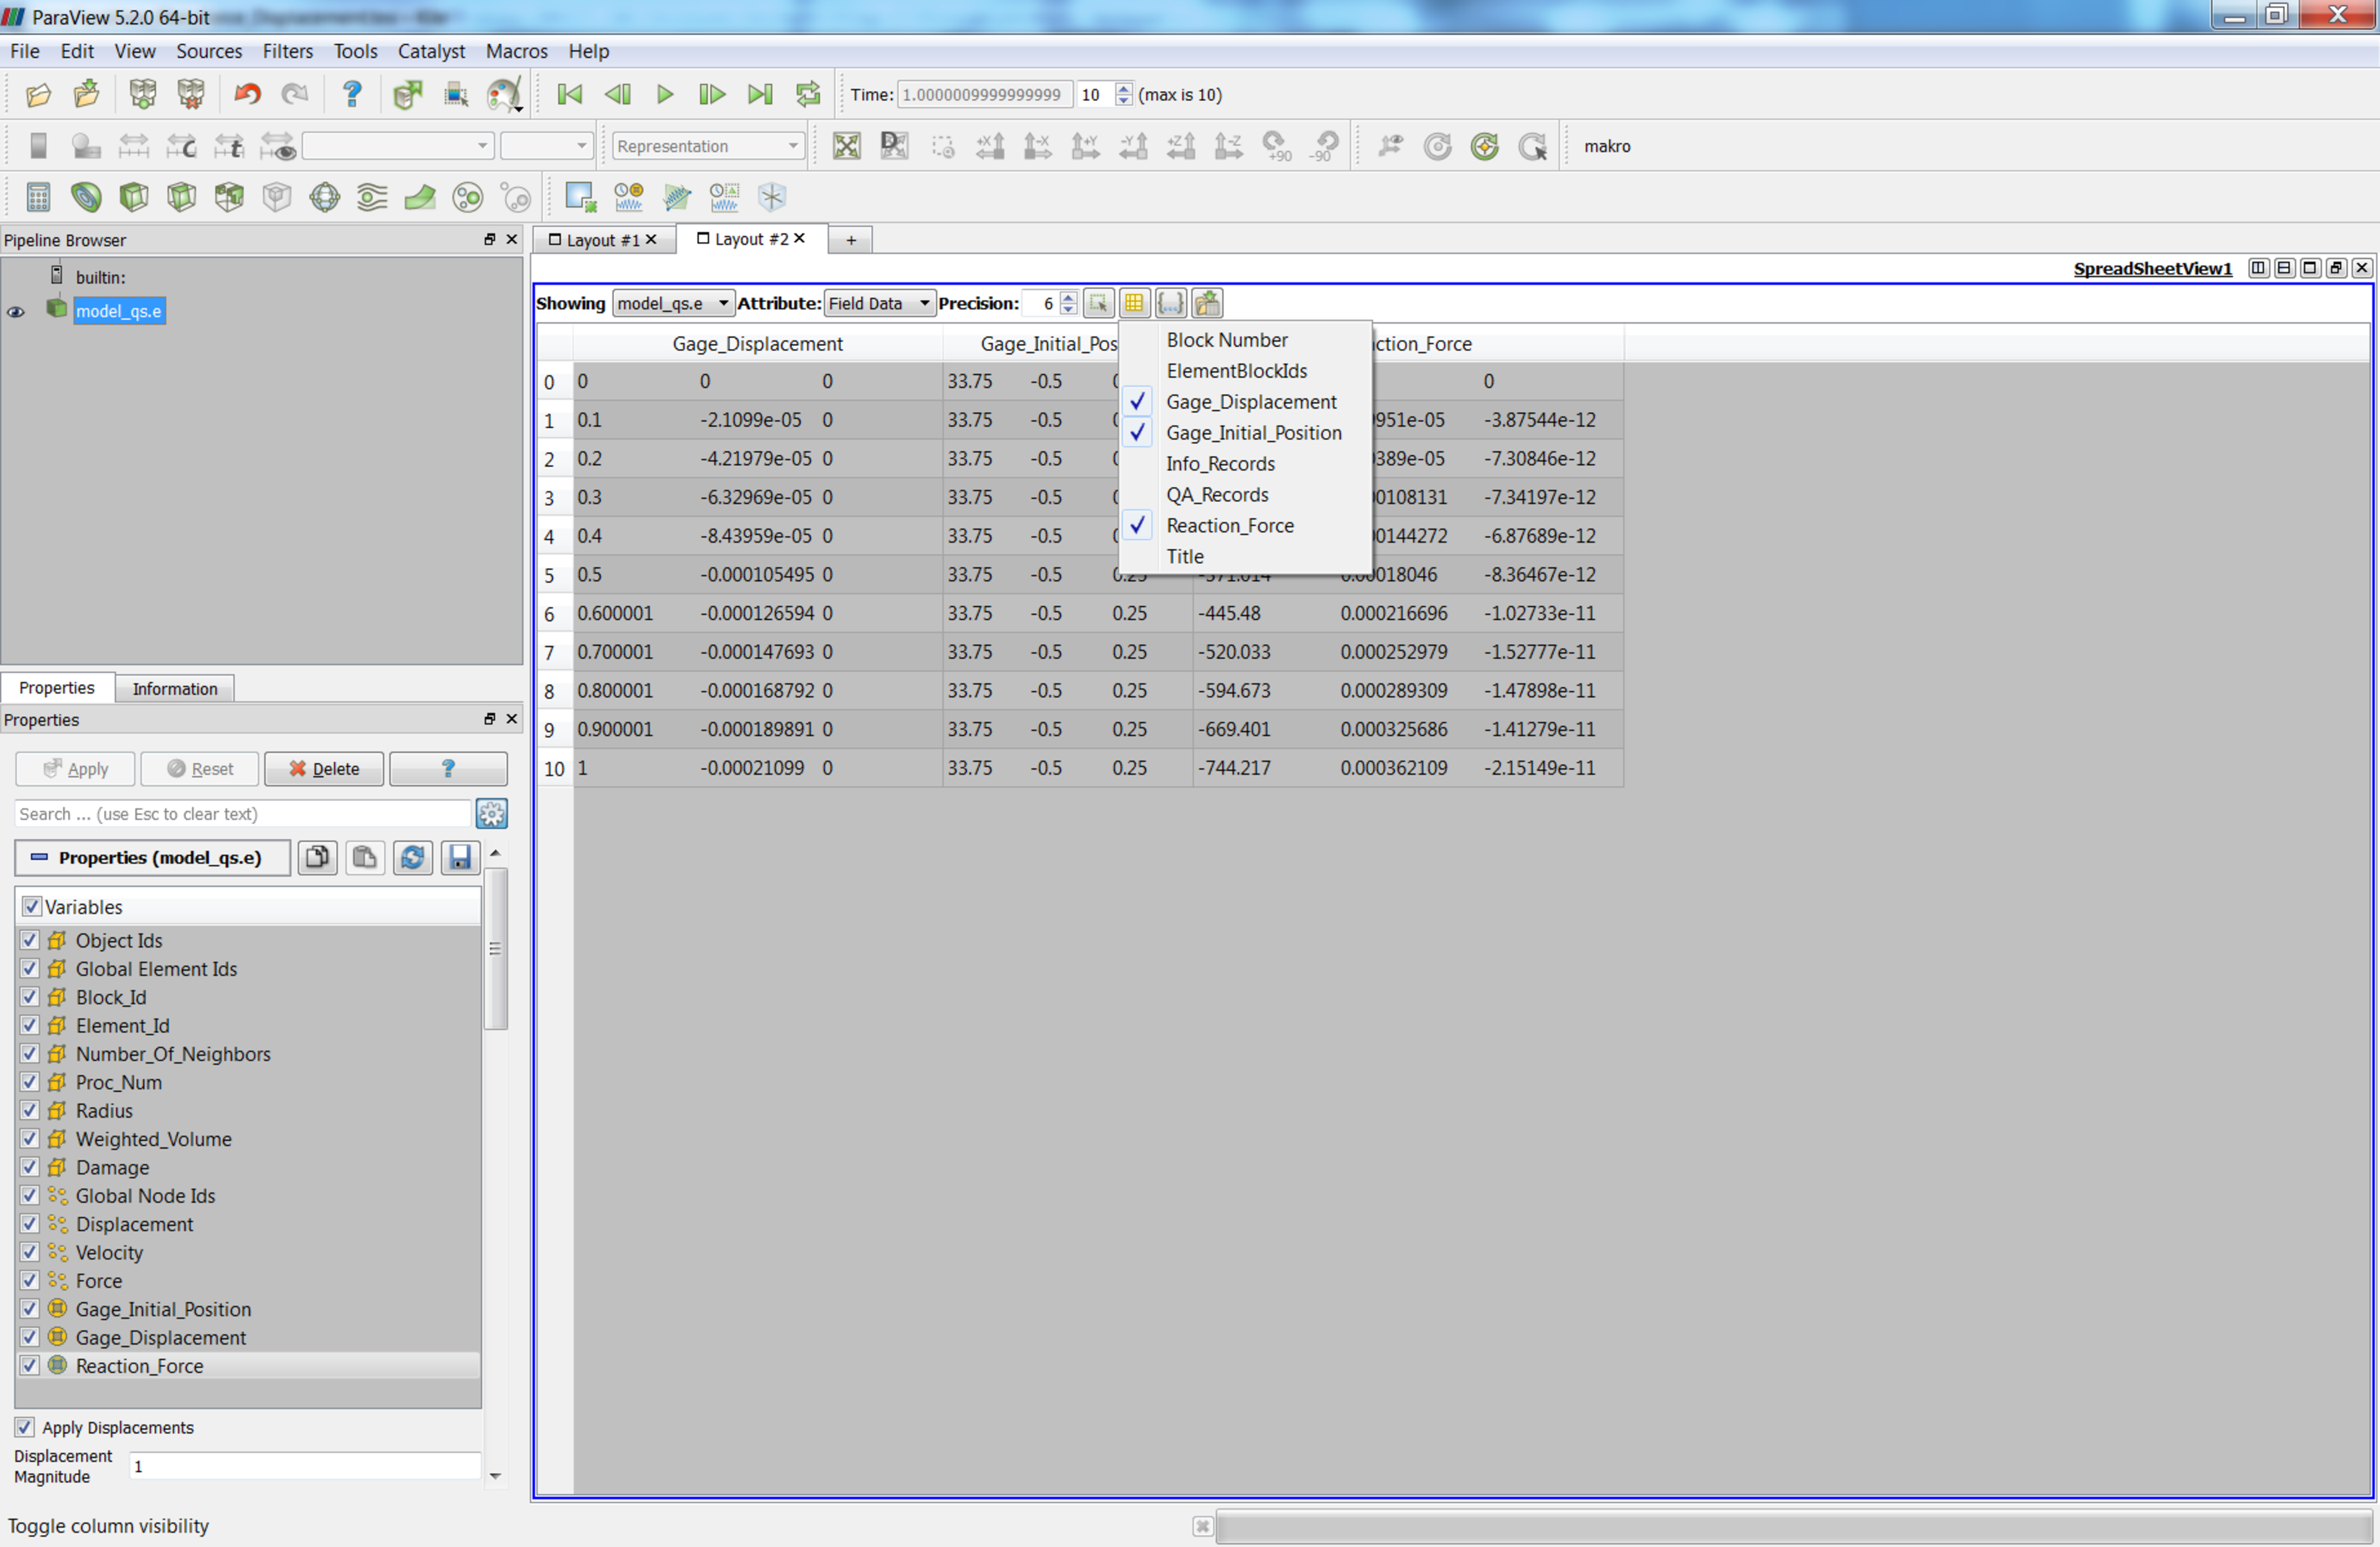
\includegraphics[width=\linewidth]{Figures/Screenshots/ParaView_ComputeClassParameter_ResultsData_2}};
      \begin{scope}[
        x={(image.south east)},
        y={(image.north west)},
      ]
        % Some label
        \node[fit={(0.22,0.785) (0.40,0.82)},myrectangularmarkup] (rect3) {};
        \node[anchor=north,mymarkuptext] (rect3label) at (rect3.south) {3};
        %
        \node[fit={(0.465,0.62) (0.585,0.82)},myrectangularmarkup] (rect4) {};
        \node[anchor=west,mymarkuptext] (rect4label) at (rect4.east) {4};
        % Help grid and labels
        %\pic{myimagegrid};
      \end{scope}
      % Outside label
    \end{tikzpicture}
    \caption{Steps 3-4}
    \label{fig:ParaView_ComputeClassParameter_ResultsData_2}
  \end{subfigure}%
\caption{Access \texttt{Compute Class Parameters} results data in \protect\paraviewname}
\label{fig:Use_ParaView_ComputeClassParameter_ResultsData}
\end{figure}

\begin{enumerate}[noitemsep]
  \item Make sure that the requested result data from the \textit{Compute Class Parameters} is available in your results file. If you are only interested in these parameters, unselect all other.
  \item Add a new view \& select \textit{SpreadSheet View}
  \item For \textit{Showing} select your model and for \textit{Attribute} select \textit{Field Data}
  \item Click 
\includegraphics[width=\iconsize]{Figures/Icons/pqRectilinearGrid16} to select the columns of interest
  \item Click 
\includegraphics[width=\iconsize]{Figures/Icons/pqSaveTable32} to save the spreadsheet data as a \texttt{csv}-file
  \begin{enumerate}[noitemsep]
    \item Specify a filename \& click \textit{Ok}
    \item In the next dialog toggle \textit{Filter Columns by Visibility}. Otherwise, all data is written to the \texttt{csv}-file.
  \end{enumerate}
  \item Do with the data whatever you want \smiley
\end{enumerate}

\levelstay{Plot result data directly in \protect\paraviewname}

\begin{figure}[htbp]
\centering
    \begin{tikzpicture}
      % External figure
      \node[anchor=south west,inner sep=0] (image) at (0,0) {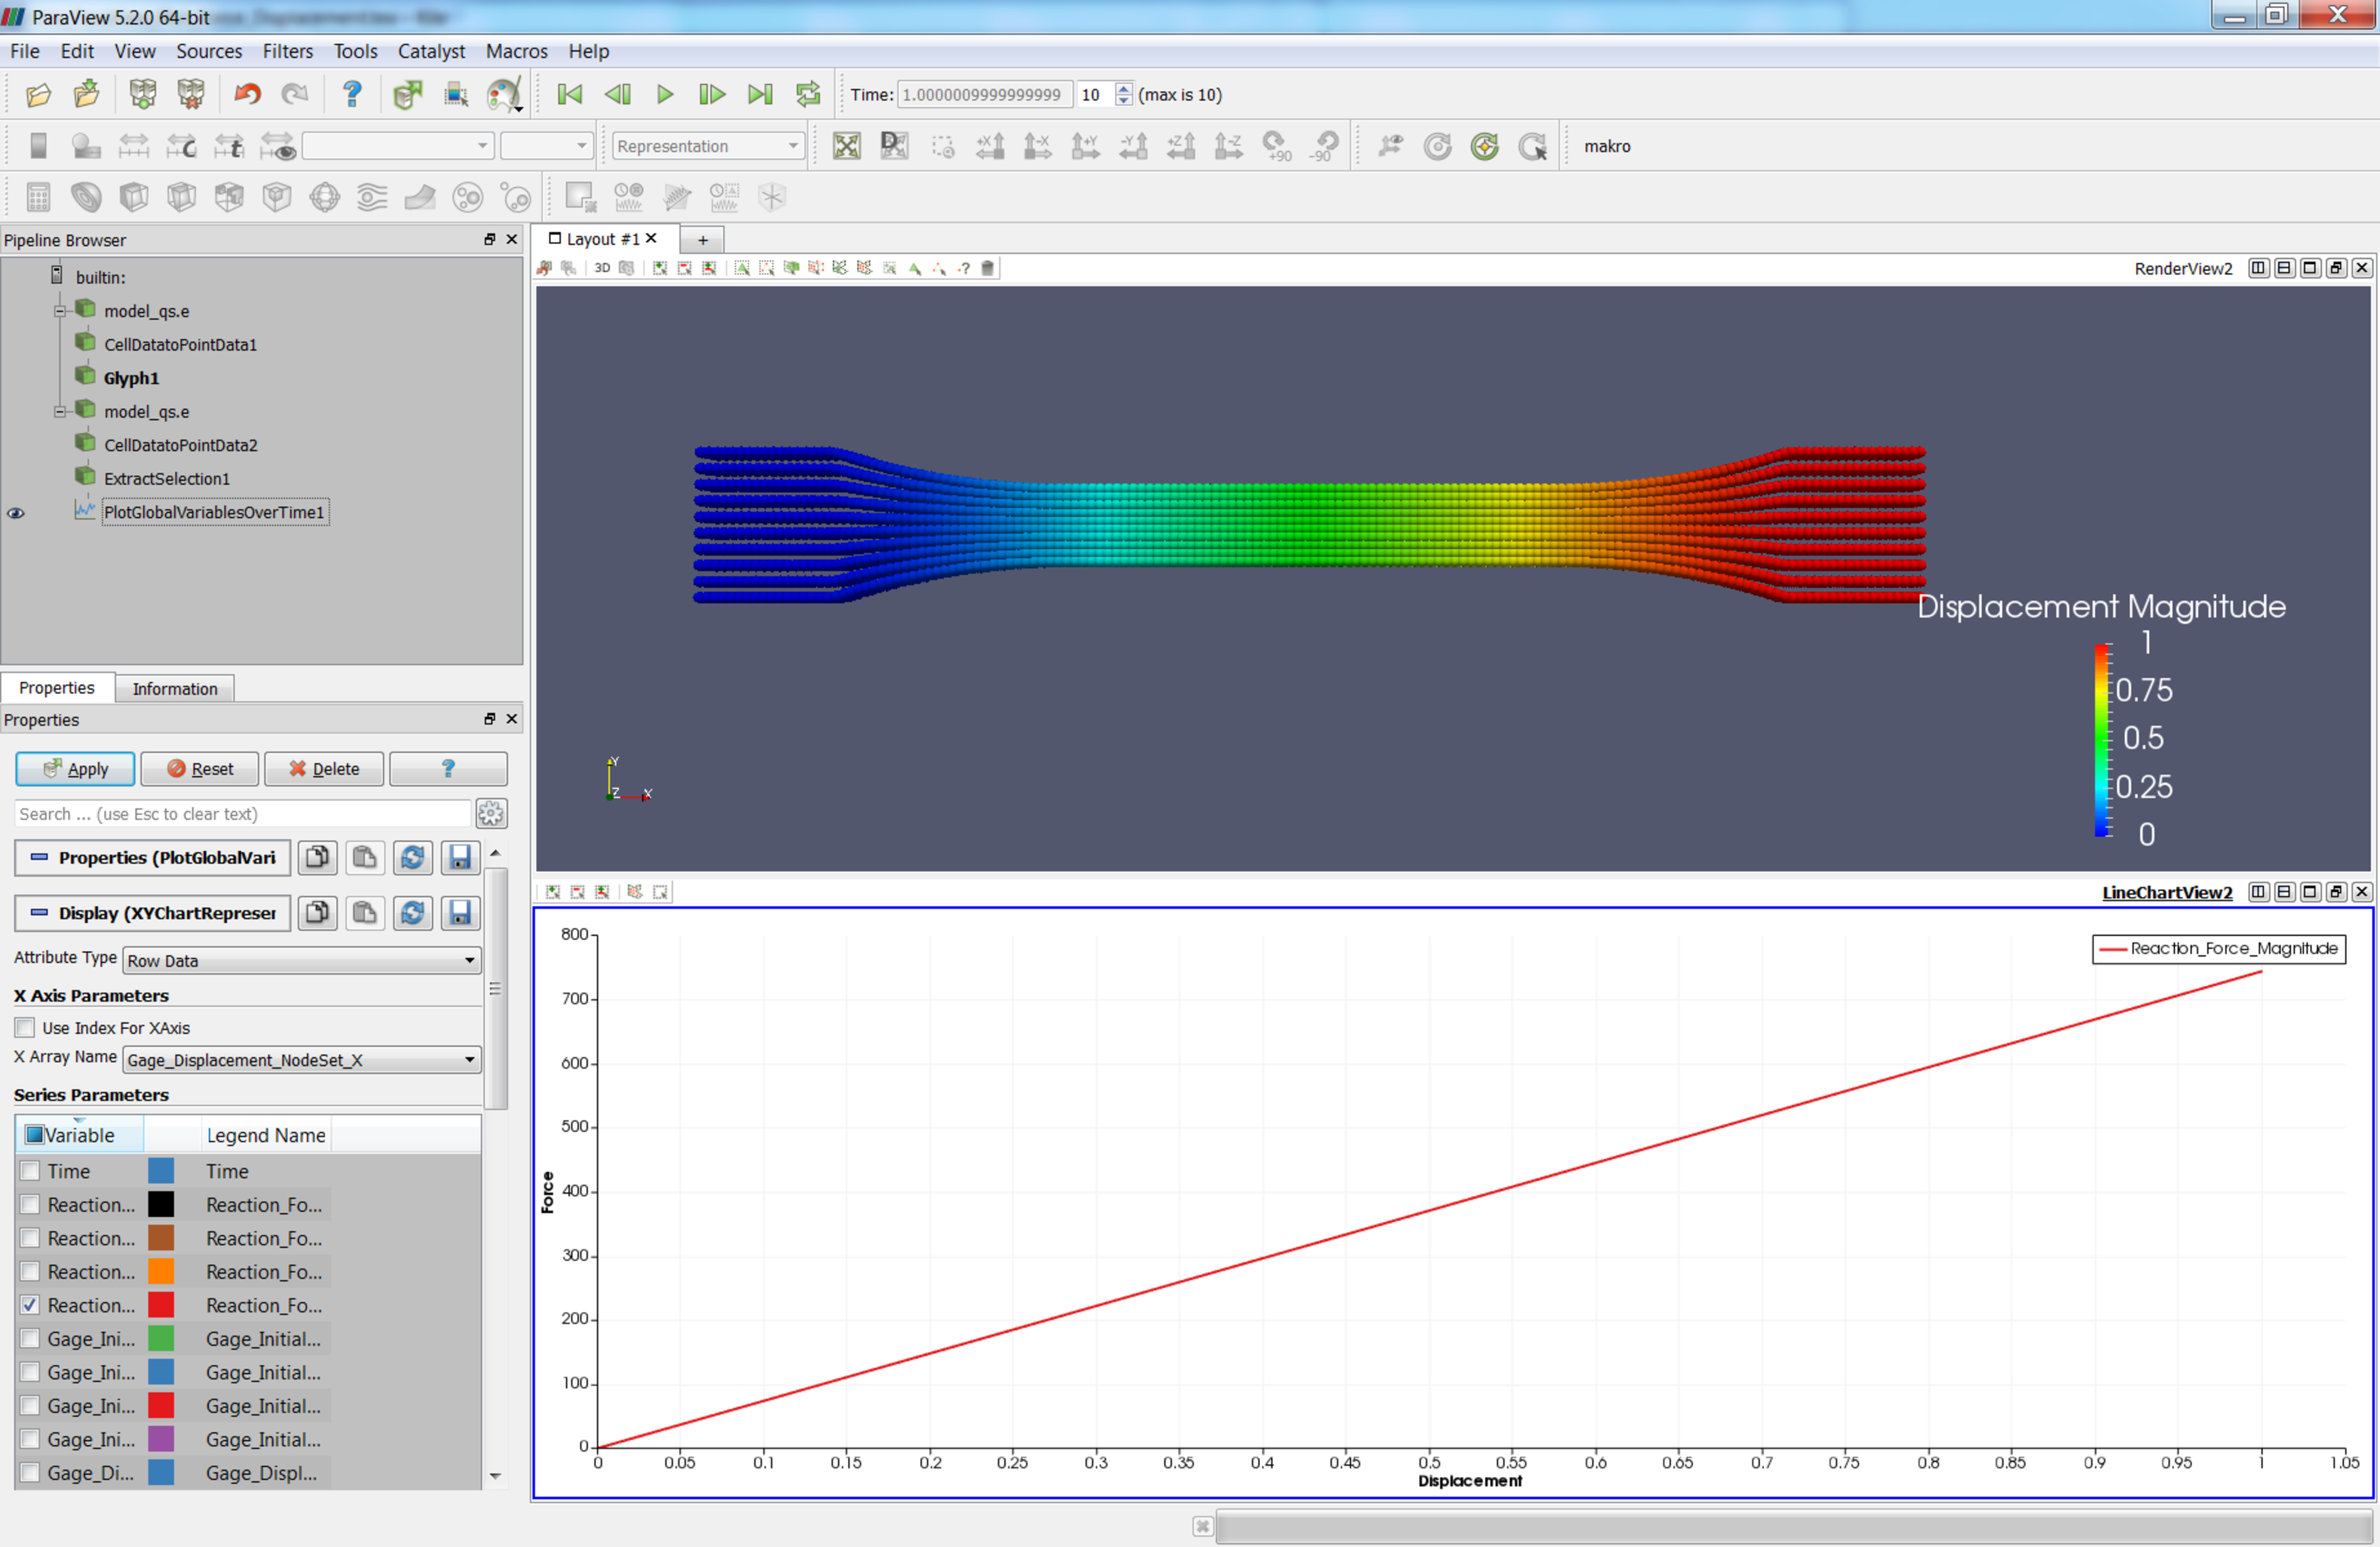
\includegraphics[width=0.8\linewidth]{Figures/Screenshots/ParaView_ComputeClassParameter_ResultsData_3}};
      \begin{scope}[
        x={(image.south east)},
        y={(image.north west)},
      ]
        % Some label
%         \node[fit={(0.007,0.10) (0.18,0.17)},myrectangularmarkup] (rect1) {};
%         \node[anchor=west,mymarkuptext] (rect1label) at (rect1.east) {1};
%         %
%         \node[fit={(0.280,0.83) (0.31,0.86)},myrectangularmarkup] (rect2) {};
%         \node[anchor=west,mymarkuptext] (rect2label) at (rect2.east) {2};
        % Help grid and labels
%         \pic{myimagegrid};
      \end{scope}
    \end{tikzpicture}
\caption{Plot \texttt{Compute Class Parameters} results data in \protect\paraviewname}
\label{fig:Use_ParaView_ComputeClassParameter_ResultsData_ForceDisplacement_in-ParaView}
\end{figure}

\begin{enumerate}[noitemsep]
  \item Import your model
  \item Make sure that the requested result data from the \textit{Compute Class Parameters} is available in your results file. If you are only interested in these parameters, unselect all other.
  \item From the menu bar:
    \begin{itemize}[noitemsep]
    \item Click Filters
    \item Click Alphabetical
    \item Click \textit{Cell Data to Point Data}
    \end{itemize}
  \item Select points of interest:
    \begin{itemize}[noitemsep]
    \item Select the \textit{Cell Data to Point Data} entry in the Pipeline Browser
    \item Create a new selection of a single or multiple points in your constraint region as described in \autoref{sec:Use_ParaView_Selection_Create}
    \item Extract the selection as described in \autoref{sec:Use_ParaView_Selection_LimitTo}
    \end{itemize}
  \item From the menu bar:
    \begin{itemize}[noitemsep]
    \item Click Filters
    \item Click Data Analysis
    \item Click \textit{Plot Selection Over Time}
    \end{itemize}
    or click 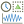
\includegraphics[width=\iconsize]{Figures/Icons/pqPlotSelectionOverTime24} in the Data Analysis toolbar
  \item Preferences in the \textit{Properties} window
    \begin{itemize}[noitemsep]
    \item Under \textit{X Axis Parameters} select your displacement component or magnitude from the \texttt{Compute Class Parameters} in the \textit{X Array Name} combobox
    \item For \textit{Series Parameters} select the force value you want to plot from the \texttt{Compute Class Parameters}, either as a component or magnitude
    \item Input a \textit{Left Axis Title} and \textit{Bottom Axis Title} if required
    \end{itemize}
  \item Click \textit{Apply}
  \item In case you want to export the chart data from here:
    \begin{itemize}[noitemsep]
    \item Left-click on the chart
    \item From the menu bar:
      \begin{itemize}[noitemsep]
      \item Click \textit{File}
      \item Click \textit{Save As}
      \item Export as \texttt{csv}-file
      \end{itemize}
    \end{itemize}
\end{enumerate}

\levelup{\protect\abaqusname}

% https://www.youtube.com/watch?v=O8CcSB11468

\leveldown{Standard}

\begin{enumerate}[noitemsep]
  \item Choose Displacement (U) \& Reaction Forces (RF) as field outputs for the step you want to have the plot
  \item Run the analysis
  \item Open the odb
  \item Reaction force over time:
  \begin{enumerate}[noitemsep]
    \item Click \textit{Create XY Data}
    \item Select Source \textit{ODB history output}
    \item Click \textit{Continue}
    \item Select all entries with beginning \textit{Reation force:} of the nodeset your are interested in
    \item Click \textit{Save as}
    \item Assign name, here ``RF'', \& in \textit{Save Operation} select \textit{sum((XY,XY,$\ldots$))}
  \end{enumerate}
  \item Displacement over time:
  \begin{enumerate}[noitemsep]
    \item Click \textit{Create XY Data}
    \item Select Source \textit{ODB history output}
    \item Click \textit{Continue}
    \item Select all entries with beginning \textit{Spatial displacement Ui:} of the nodeset your are interested in
    \item Click \textit{Save as}
    \item Assign name, here ``U'', \& in \textit{Save Operation} select \textit{avg((XY,XY,$\ldots$))}
  \end{enumerate}
  \item Reaction force over displacement:
  \begin{enumerate}[noitemsep]
    \item Click \textit{Create XY Data}
    \item Select Source \textit{Operate on XY data}
    \item Click \textit{Continue}
    \item From \textit{Operators} select \textit{Combine}
    \item In the equation, at first select ``U'', than ``RF'', the equation than should be \verb+combine ("U","F")+
    \item Select \textit{Plot Expression}
  \end{enumerate}
\end{enumerate}

\levelstay{Explicit}

\begin{enumerate}[noitemsep]
  \item Choose Displacement (U), Reaction Forces (RF) \& Nodal forces (NFORC) as field outputs for the step you want to have the plot
  \item Run the analysis
  \item Open the odb
  \item Reaction force \& Displacement over time:
  \begin{enumerate}[noitemsep]
    \item Click \textit{Create XY Data}
    \item Select Source \textit{ODB field output}
    \item Click \textit{Continue}
    \item \textit{XY Data from ODB Field Output} dialog:
      \begin{enumerate}[noitemsep]
        \item In the \textit{Variables} tab, select \textit{Unique nodal} in the \textit{Position} combobox and all necessary entry checkboxes, here RF1 and U1
        \item In the \textit{Elements/Nodes} tab, select the requested nodeset
      \end{enumerate}
    \item Click \textit{Save}
  \end{enumerate}
  \item Sum forces:
  \begin{enumerate}[noitemsep]
    \item Click \textit{Create XY Data}
    \item Select Source \textit{Operate on XY data}
    \item From \textit{Operators} select \textit{sum}
    \item In the equation, select all ``RF1'' entries`` and click \textit{Add to expression}
    \item Click \textit{Save as} \& assign name ''RF``
  \end{enumerate}
  \item Average displacements:
  \begin{enumerate}[noitemsep]
    \item Click \textit{Create XY Data}
    \item Select Source \textit{Operate on XY data}
    \item From \textit{Operators} select \textit{avg}
    \item In the equation, select all ``U1'' entries`` and click \textit{Add to expression}
    \item Click \textit{Save as} \& assign name ''U``
  \end{enumerate}
  \item Reaction force over displacement:
  \begin{enumerate}[noitemsep]
    \item Click \textit{Create XY Data}
    \item Select Source \textit{Operate on XY data}
    \item Click \textit{Continue}
    \item From \textit{Operators} select \textit{Combine}
    \item In the equation, at first select ``U'', than ``RF'', the equation than should be \verb+combine ("U","F")+
    \item Select \textit{Plot Expression}
  \end{enumerate}
\end{enumerate}

\levelstay{Save XY data}

\begin{enumerate}[noitemsep]
  \item Open the odb
  \item Create all results
  \item In the menu bar, click \textit{Report}
  \item Click \textit{XY}
  \item Adjust the dialog preferences according to your needs
\end{enumerate}